\documentclass[12pt,a4paper]{article}

% ---------------------------------------------------------
% Packages
% ---------------------------------------------------------
\usepackage[a4paper,
            left=1in,
            right=1in,
            top=0.8in,
            bottom=0.8in]{geometry}

\usepackage{newtxtext}
\usepackage{newtxmath}
\usepackage{pgfgantt}
\usepackage{graphicx}
\usepackage{amssymb}
\usepackage{array}
\usepackage{tabularx}
\usepackage{longtable}
\usepackage{booktabs}
\usepackage{multirow}
\usepackage{enumitem}
\usepackage{setspace}
\usepackage{fancyhdr}
\usepackage{titlesec}
\usepackage{caption}
\usepackage{float}
\usepackage{amssymb}
\usepackage{pifont}
\usepackage{ragged2e}
\usepackage{url}
\usepackage[hidelinks]{hyperref}

% ---------------------------------------------------------
% General Formatting
% ---------------------------------------------------------
\setlength{\parindent}{0pt}
\setlength{\parskip}{6pt}

\onehalfspacing

% Section formatting
\titleformat{\section}
  {\bfseries\large}
  {\thesection.}
  {0.5em}
  {}

\titlespacing*{\section}
  {0pt}
  {12pt}
  {6pt}

% ---------------------------------------------------------
% Header / Footer
% ---------------------------------------------------------
\pagestyle{fancy}
\fancyhf{}

\fancyfoot[R]{\thepage\;|\;P a g e}

\renewcommand{\headrulewidth}{0pt}
\renewcommand{\footrulewidth}{0pt}

% ---------------------------------------------------------
% Table formatting
% ---------------------------------------------------------
\renewcommand{\arraystretch}{1.25}

% ---------------------------------------------------------
% Custom commands
% ---------------------------------------------------------

% Green check mark similar to the original template
\newcommand{\greencheck}{%
    \colorbox{green!50}{\Large\checkmark}%
}

% ---------------------------------------------------------
% Document
% ---------------------------------------------------------
\begin{document}

% =========================================================
% COVER PAGE
% =========================================================

\begin{titlepage}
\thispagestyle{empty}

\begin{center}

\IfFileExists{vu_logo.png}{
    
\includegraphics[width=1.0in]{vu_logo.png}
    \vspace{0.2in}
}{}

{\Large\bfseries Varendra University}

\vspace{0.08in}

{\large\bfseries Department of Computer Science and Engineering}

\vspace{0.55in}

{\large\bfseries Undergraduate Thesis Proposal}

\vspace{0.55in}

{\large\bfseries Development of a Taxonomically Verified Image Dataset for\\[4pt] Bangladeshi Fish Species}

\vfill

{\bfseries Submitted by:}

\vspace{0.25in}

Sahariar Ahmed Isteyak (232311289)\\
Most. Amrin Akter (232311246)\\
Lamia Hasan (232311251)

\vspace{0.25in}

\textbf{Program:} B.Sc. in Computer Science and Engineering\\
\textbf{Semester:} 7th\\
\textbf{Section:} D\\
\textbf{Course Code:} CSE 4100\\
\textbf{Course Title:} Project or Thesis with Seminar Part I

\vfill

{\bfseries Supervisor:}

\vspace{0.08in}

Zuairia Raisa Bintay Makin\\
Lecturer\\
Department of Computer Science and Engineering

\vfill

{\bfseries Submission Date:} 07 October 2026

\end{center}

\end{titlepage}


% =========================================================
% PAGE 2
% =========================================================

\setcounter{page}{1}
\tableofcontents
\newpage

\section{Introduction}

Bangladesh is strongly connected to inland and open-water fisheries through rivers, ponds, beels, floodplains, haors and other aquatic habitats. The Department of Fisheries identifies inland fisheries as a major national resource and reports 260 freshwater fish species in the country. This diversity creates an important opportunity for computer-vision research, but it also creates a data-quality challenge: a recognition system is only as dependable as the images and labels used to train and evaluate it.

Fish identification from images is difficult because species can share similar body shapes, colors, fin structures, scale patterns, and visual features. Lighting, water condition, background, camera angle, fish orientation, and image quality can further change the appearance of the same species. Existing Bangladesh-focused datasets show that image-based fish recognition is already an active research direction. For example, BD-Freshwater-Fish contains 4,389 images of 12 species, while a later smartphone-based dataset contains 24,925 images of 21 freshwater species.

FishBD is proposed not simply as a larger collection of pictures, but as a curated research resource in which species identity, source information, image quality, metadata, and validation status are treated as linked components. The project will combine field/source collection, taxonomic verification, annotation, preprocessing, and AI-assisted quality screening into one reproducible pipeline.

\textbf{Why this topic is important in the Bangladesh context:}
\begin{itemize}
    \item Fisheries have a direct national importance: the Department of Fisheries reports 2.53\% contribution to national GDP and 22.26\% to agricultural GDP in 2023--24.
    \item Bangladesh contains substantial freshwater fish diversity, making local rather than generic international datasets important for local recognition tasks.
    \item The national Red List assessment included 253 freshwater fish species and identified conservation concerns associated with habitat loss, overexploitation, invasive species, pollution and climate change.
    \item Computer-vision systems can support identification and monitoring, but their reliability depends strongly on representative images and correct labels.
    \item Students, researchers and fisheries-related users need datasets that can be inspected, reused, and understood through clear metadata rather than opaque collections of images.
\end{itemize}

\textbf{Scope of the proposed work:}
\begin{itemize}
    \item Focus on Bangladeshi freshwater fish species selected according to feasibility, availability and taxonomic relevance.
    \item Collect or curate images representing multiple environments and realistic visual variation rather than a single controlled background only.
    \item Attach scientific name, local name, source/habitat information, image identifier and verification status to each accepted image.
    \item Use ML/DL as an assistive screening and benchmarking component, while keeping human/taxonomic verification as the final authority.
    \item Produce documentation and dataset statistics so future researchers can understand how the dataset was constructed.
\end{itemize}

\section{Literature Review / Background Study}

Recent Bangladesh-focused work demonstrates strong interest in fish image classification, but the studies also reveal why dataset construction remains a meaningful research problem.

\textbf{Research gap:} The literature shows that Bangladesh already has useful fish-image resources, so FishBD should not claim that no dataset exists. The more defensible gap is methodological: existing resources differ in species scope, collection conditions, metadata depth and validation procedures. FishBD therefore focuses on creating a transparent dataset-development framework in which taxonomic verification is explicitly documented and ML/DL is used for quality assistance rather than treated as a substitute for taxonomic expertise.

\textbf{Taxonomic reference basis:} FishBase currently lists hundreds of fish species for Bangladesh and provides scientific classification and identification-oriented information. The IUCN Red List of Bangladesh separately documents the conservation status of freshwater fishes. These sources can support the reference layer used for scientific names and conservation context.

\begin{table}[H]
\centering
\caption{Comparative summary of related work.}
\small
\begin{tabularx}{\textwidth}{|p{1.2in}|p{1.0in}|X|p{1.5in}|}
\hline
\textbf{Existing work} & \textbf{Scale / coverage} & \textbf{Main contribution} & \textbf{Gap relevant to FishBD} \\
\hline
BD-Freshwater-Fish (2024) \cite{ref2} & 4,389 images; 12 species & Bangladesh freshwater fish image dataset captured with HD mobile cameras. & Limited species coverage and dataset scope; primarily designed for AI classification/detection. \\
\hline
Smartphone freshwater dataset (2025) \cite{ref3} & 24,925 images; 21 species & Large labeled smartphone dataset with variation in lighting/background. & Useful scale, but FishBD adds a stronger emphasis on explicit taxonomic verification and a human-AI quality loop. \\
\hline
SmallFishBD (2025) \cite{ref4} & 10 native small-fish species & Curated native small-fish dataset with standardized imaging and augmentation. & Focused on a specific small-fish group and controlled collection context. \\
\hline
Bangladeshi DL classification (2023) \cite{ref5} & 8 species in a new dataset & Benchmarked pretrained CNN architectures and a CNN+ConvLSTM approach. & Demonstrates model capability, but the dataset-verification problem remains separate from model accuracy. \\
\hline
\end{tabularx}
\end{table}

\section{Problem Statement}

Bangladesh has substantial freshwater fish diversity, but image-based fish recognition is constrained by the quality, representativeness and reliability of available training data. Existing datasets are valuable but vary in species coverage and collection design. Images may come from markets or controlled backgrounds, and the same species may appear differently under changes in orientation, lighting, background, and image quality.

The central problem addressed by FishBD is therefore the absence of a clearly documented, taxonomically verified and quality-controlled dataset-development pipeline that connects image collection with authoritative species identity, metadata, AI-assisted screening and human feedback. Without such a process, an apparently accurate ML/DL model may learn from mislabeled, duplicated, biased or visually unrepresentative examples.

\textbf{Research question:}
How can a Bangladesh-focused fish image dataset be constructed so that species labels are taxonomically defensible, image quality is controlled, metadata are standardized, and ML/DL can assist---rather than replace---human verification?


\section{Objectives}

\begin{itemize}[leftmargin=0.35in]
    \item Design and implement a reproducible pipeline for collecting and curating images of selected Bangladeshi freshwater fish species.
    \item Verify each accepted species label against recognized taxonomic references and expert feedback, recording the verification status as dataset metadata.
    \item Apply standardized quality control, duplicate screening, annotation and preprocessing so that the final dataset is suitable for machine-learning and deep-learning research.
    \item Develop an ML/DL-assisted screening stage that flags low-confidence, visually inconsistent or potentially mislabeled samples for human re-checking.
    \item Produce a documented benchmark-ready dataset with defined training, validation and test partitions, along with dataset statistics and quality reports.
\end{itemize}


\section{Proposed Methodology / System Design}

\begin{figure}[H]
\centering
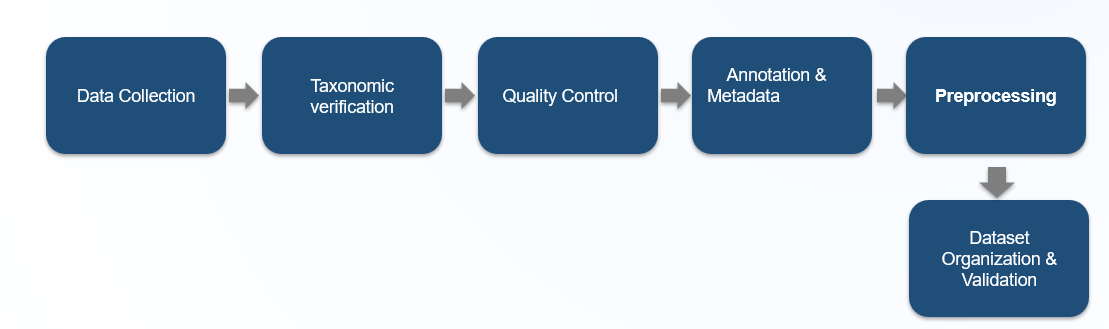
\includegraphics[width=0.9\textwidth]{figures/image2.png}
\caption{System architecture and proposed dataset development pipeline.}
\label{fig:system_design}
\end{figure}

\subsection{Stage A — Source and image collection}
Collect images from feasible sources such as field locations, fish markets, fisheries-related contacts, institutional collections and openly reusable sources, subject to permission and usage conditions. Record source, approximate collection context, date where available, local name, provisional identification and image identifier. Seek variation in orientation, distance, lighting, background and body presentation.

\subsection{Stage B — Taxonomic verification}
Taxonomic verification will follow a hierarchy. First, the provisional species identity will be compared with authoritative taxonomic resources such as FishBase \cite{ref6}. Second, morphological characteristics visible in the image will be checked against the expected species description. Third, uncertain cases will be reviewed by a knowledgeable human reviewer or taxonomic expert where available.

\subsection{Stage C — Quality control and annotation}
Remove exact or near-duplicate images where they could cause data leakage. Flag or remove severely blurred, overexposed, underexposed, obstructed or unusable images. Maintain a consistent image naming convention and unique image ID. Store scientific name, local/common name, source/habitat, location when appropriate, verification status and other available metadata.

\subsection{Stage D — ML/DL-assisted screening}
After a sufficiently verified subset is available, a baseline classifier can be trained using CNN architectures or a Vision Transformer (ViT)-type model. The purpose at this stage is not to declare the taxonomic truth automatically. Instead, the model can identify samples that deserve additional inspection.

\textbf{Verification feedback mechanism:} The feedback mechanism is intentionally conservative. A model disagreement is treated as a signal for inspection, not proof that the human label is wrong.

\subsection{Dataset organization and validation}
Create training, validation and test partitions at the specimen/source level where possible, reducing the chance that near-identical images of one fish appear in multiple splits. Report class distribution, image counts, source distribution, image-quality statistics and verification status.


\section{Method Justification}

The proposed methodology fits the project because the core deliverable is a reliable dataset, not merely a classification model. A dataset-first approach allows the project to address label correctness, diversity, metadata quality and reproducibility before measuring AI performance.

\begin{table}[H]
\centering
\caption{Design choices and justification.}
\small
\begin{tabularx}{\textwidth}{|p{1.3in}|X|p{1.3in}|}
\hline
\textbf{Design choice} & \textbf{Why it is suitable} & \textbf{Expected effect} \\
\hline
Taxonomic reference + human review & Species names require domain knowledge and authoritative classification; AI confidence alone is insufficient. & Higher label defensibility. \\
\hline
Diverse image collection & Fish appearance changes with habitat, orientation, lighting and background. & Better representation of real use conditions. \\
\hline
Quality-control log & Explicit acceptance/rejection criteria make curation auditable. & More reproducible dataset construction. \\
\hline
ML/DL-assisted screening & Models can identify hard or unusual samples at scale after a verified seed set exists. & Efficient identification of cases needing review. \\
\hline
Source-aware split & Related images can create leakage if randomly split. & More credible future model evaluation. \\
\hline
\end{tabularx}
\end{table}


\section{Expected Outcomes}

\begin{itemize}[leftmargin=0.35in]
    \item A structured FishBD image dataset covering selected Bangladeshi freshwater fish species.
    \item Taxonomically supported scientific and local/common names with verification status.
    \item High-quality images representing more than one collection context where feasible.
    \item Standardized metadata, data dictionary, and quality-control rejection records.
    \item Baseline ML/DL screening results showing how model confidence can support human review.
    \item Training, validation and test partitions suitable for future fish-recognition experiments.
\end{itemize}


\section{Tools and Technologies to Be Used}

\begin{table}[H]
\centering
\caption{Tools and Technologies.}
\small
\begin{tabularx}{\textwidth}{|p{1.0in}|p{1.2in}|X|p{1.2in}|}
\hline
\textbf{Category} & \textbf{Tool / technology} & \textbf{Purpose} & \textbf{Why selected} \\
\hline
Programming & Python & Data processing, automation and experiments & Widely used for CV and data science. \\
\hline
Image processing & OpenCV / Pillow & Resize, format conversion, quality checks & Open-source and suitable for batch image processing. \\
\hline
Data handling & Pandas / NumPy & Metadata tables, statistics and preprocessing & Efficient structured data manipulation. \\
\hline
Annotation & CVAT / Label Studio & Image annotation and review workflow & Supports structured labeling and curation. \\
\hline
ML/DL & PyTorch / TensorFlow; CNN / ViT models & Baseline recognition and screening & Flexible research ecosystem. \\
\hline
Development & VS Code / Colab & Coding and experimental work & Accessible development. \\
\hline
Metadata & CSV / JSON & Portable dataset records & Simple, transparent and reusable formats. \\
\hline
Taxonomy references & FishBase; IUCN & Scientific identity and biodiversity context & Provides external reference information for verification. \\
\hline
\end{tabularx}
\end{table}


\section{Work Division and Team Management}

The three members will work without a separate team-leader role. Responsibilities are divided by primary ownership, while verification decisions and major dataset changes are discussed jointly.

\begin{table}[H]
\centering
\caption{Work Division and Team Management}
\label{tab:work-division}
\begin{tabularx}{\textwidth}{|p{1.5in}|X|p{1.5in}|}
\hline
\textbf{Team Member} & \textbf{Assigned Tasks} & \textbf{Shared Responsibility} \\
\hline
Sahariar Ahmed Isteyak (232311289) & Source coordination, image collection records, dataset pipeline & Literature review, testing and final review \\
\hline
Most. Amrin Akter (232311246) & Scientific/local name checking, annotation, metadata verification & Expert feedback coordination and documentation \\
\hline
Lamia Hasan (232311251) & Quality control, preprocessing, duplicate checks, dataset statistics & ML/DL screening and final audit \\
\hline
\end{tabularx}
\end{table}


\section{Timeline}

The schedule is deliberately overlapping because collection, verification, quality control and annotation are iterative. Field availability and expert-review timing may require adjustments without changing the overall 12-month completion target.

\begin{figure}[H]
\centering
\resizebox{\textwidth}{!}{%
\begin{ganttchart}[
    hgrid,
    vgrid,
    x unit=1.0cm,
    y unit title=0.7cm,
    y unit chart=0.65cm,
    title height=1,
    bar height=0.5,
    bar label font=\small,
    title label font=\small\bfseries
]{1}{12}

\gantttitle{Thesis Research Timeline}{12} \\

\gantttitle{M1}{1}
\gantttitle{M2}{1}
\gantttitle{M3}{1}
\gantttitle{M4}{1}
\gantttitle{M5}{1}
\gantttitle{M6}{1}
\gantttitle{M7}{1}
\gantttitle{M8}{1}
\gantttitle{M9}{1}
\gantttitle{M10}{1}
\gantttitle{M11}{1}
\gantttitle{M12}{1} \\

\ganttbar{Planning \& literature review}{1}{2} \\
\ganttbar{Dataset design \& protocol}{2}{3} \\
\ganttbar{Image/source collection}{3}{6} \\
\ganttbar{Taxonomic verification}{4}{7} \\
\ganttbar{Quality control \& duplicate screening}{6}{8} \\
\ganttbar{Annotation \& metadata}{7}{9} \\
\ganttbar{Preprocessing \& dataset org.}{8}{10} \\
\ganttbar{ML/DL baseline \& screening}{9}{10} \\
\ganttbar{Feedback \& re-verification}{10}{11} \\
\ganttbar{Validation \& analysis}{11}{12} \\
\ganttbar{Documentation \& final report}{11}{12}

\end{ganttchart}%
}
\caption{Proposed 12-Month Thesis Timeline}
\label{fig:thesis_timeline}
\end{figure}


\section{Cost-Benefit Analysis}

The project is designed as a low-cost research activity because it can use existing smartphones/cameras, open-source software and available computing resources. The main variable cost is expected to be local travel and field collection.

\begin{table}[H]
\centering
\caption{Cost Control Strategy.}
\small
\begin{tabularx}{\textwidth}{|p{1.2in}|X|X|}
\hline
\textbf{Cost area} & \textbf{Expected requirement} & \textbf{Cost-control strategy} \\
\hline
Field travel & Transport to selected collection locations & Prioritize nearby feasible sites and combine visits. \\
\hline
Image capture & Existing smartphones/cameras where adequate & Avoid dedicated camera purchase unless quality requires it. \\
\hline
Software & Python, OpenCV, CVAT, Label Studio & Prefer open-source tools. \\
\hline
Compute & Local PC and/or free/available cloud resources & Use efficient baselines and shared experiments. \\
\hline
Storage & Local drive + available cloud storage & Store compressed working copies and retain organized master records. \\
\hline
\end{tabularx}
\end{table}


\section{Constraints and Limitations}

\begin{itemize}[leftmargin=0.35in]
    \item \textbf{Economic:} Travel budget may restrict geographic coverage.
    \item \textbf{Environmental:} Weather and water conditions can affect field collection. Some species may be seasonally available or difficult to photograph.
    \item \textbf{Ethical and social:} Permission may be required for photographs or institutional sources. Images and metadata must respect source ownership and responsible data sharing.
    \item \textbf{Technical:} Poor lighting, occlusion, blur and background variation can reduce image quality. Class imbalance may occur when some species are easier to obtain than others.
    \item \textbf{Taxonomic:} Some images may not contain enough diagnostic features for confident identification. Expert availability may be limited.
\end{itemize}


\section{Societal Impact}

\begin{itemize}[leftmargin=0.35in]
    \item \textbf{Education:} Students can use a Bangladesh-focused dataset to learn computer vision, curation and fish identification.
    \item \textbf{Research:} Researchers can reuse standardized images and metadata for classification and biodiversity studies.
    \item \textbf{Fisheries:} Reliable visual references may support future digital tools for fish monitoring.
    \item \textbf{Conservation:} Better species records can contribute to computational biodiversity studies.
    \item \textbf{Responsible AI:} Separating taxonomic authority from model prediction reduces the risk of presenting an AI guess as biological truth.
\end{itemize}


\section{Complex Engineering Problem Mapping}

FishBD maps to the complex engineering problem domains because the work is not a single coding task. It combines biological knowledge, data engineering, image processing, AI, field constraints, stakeholder interaction and validation requirements.

\begin{table}[H]
\centering
\caption{Mapping with complex problem solving.}
\label{tab:complex-problem}
\small
\renewcommand{\arraystretch}{1.3}
\begin{tabularx}{\textwidth}{|>{\centering\arraybackslash}X|>{\centering\arraybackslash}X|>{\centering\arraybackslash}X|>{\centering\arraybackslash}X|>{\centering\arraybackslash}X|>{\centering\arraybackslash}X|>{\centering\arraybackslash}X|}
\hline
\textbf{WP1} & \textbf{WP2} & \textbf{WP3} & \textbf{WP4} & \textbf{WP5} & \textbf{WP6} & \textbf{WP7} \\
\hline
Depth of Knowledge & Range of Conflicting Req. & Depth of Analysis & Familiarity of Issues & Applicable Codes & Stakeholder Inv. & Interdependence \\
\hline
{\Large\checkmark} & {\Large\checkmark} & {\Large\checkmark} & {\Large\checkmark} & & {\Large\checkmark} & {\Large\checkmark} \\
\hline
\end{tabularx}
\end{table}


\section{Complex Engineering Activity Mapping}

The proposal aligns most strongly with EA1, EA2, EA3 and EA4. EA5 is also relevant because the project combines familiar programming techniques with less predictable field and taxonomic situations.

\begin{table}[H]
\centering
\caption{Mapping with complex engineering activities.}
\label{tab:complex-activity}
\small
\renewcommand{\arraystretch}{1.3}
\begin{tabularx}{\textwidth}{|>{\centering\arraybackslash}X|>{\centering\arraybackslash}X|>{\centering\arraybackslash}X|>{\centering\arraybackslash}X|>{\centering\arraybackslash}X|}
\hline
\textbf{EA1} & \textbf{EA2} & \textbf{EA3} & \textbf{EA4} & \textbf{EA5} \\
\hline
Range of resources & Level of Interaction & Innovation & Consequences & Familiarity \\
\hline
{\Large\checkmark} & {\Large\checkmark} & {\Large\checkmark} & {\Large\checkmark} & {\Large\checkmark} \\
\hline
\end{tabularx}
\end{table}


\section{Green Computing Considerations}
\begin{itemize}[leftmargin=0.35in]
    \item Prefer efficient baseline models before large-scale deep-learning experiments.
    \item Use pretrained models and transfer learning where appropriate to reduce unnecessary training computation.
    \item Use shared and reusable datasets so future researchers do not need to repeat the same image-collection effort.
    \item Use free/open-source software where possible to reduce hardware and licensing overhead.
\end{itemize}


\section{Lifelong Learning and Personal Development}
\begin{itemize}[leftmargin=0.35in]
    \item Develops practical skills in dataset engineering, image preprocessing and computer-vision experimentation.
    \item Builds an understanding of how scientific taxonomy and AI-based classification can complement each other.
    \item Improves research skills through literature review, source evaluation, citation, documentation and reproducibility.
    \item Strengthens teamwork and communication through shared review and feedback.
\end{itemize}


\section{References}

\begin{enumerate}
    \item \label{ref1} Department of Fisheries, Bangladesh, ``Fisheries Sector: Prospects and Potentials / Fish Production,'' updated June 23, 2025.
    \item \label{ref2} P. K. Das et al., ``BD-freshwater-fish: An image dataset from Bangladesh for AI-powered automatic fish species classification,'' Data in Brief, vol. 57, 111132, 2024.
    \item \label{ref3} S. Sunny et al., ``Comprehensive smartphone image dataset for fish species identification in Bangladesh's freshwater ecosystems,'' Data in Brief, vol. 61, 111629, 2025.
    \item \label{ref4} M. H. Ferdaus et al., ``SmallFishBD: An extensive image dataset of common native small fish species in Bangladesh,'' Data in Brief, vol. 63, 112193, 2025.
    \item \label{ref5} ``An advanced Bangladeshi local fish classification system based on the combination of deep learning and IoT,'' Journal of Agriculture and Food Research, vol. 14, 100663, 2023.
    \item \label{ref6} FishBase, ``Fish Species in Bangladesh,'' online database, accessed October 2026.
\end{enumerate}

\end{document}
